
\label{sect:application}

\note{Start by describing the training and test sets here.
Mention their redshift and magnitude ranges.
Calculate the min and max wavelength of the training set, and say that we will try to reconstruct spectra over that wavelength range.}




\subsection{The Training and Test Set}

\note{Move discussion of the training and test set here.}




\subsection{Training Templates on the Data}

Eight naive templates were chosen to represent the underlying SED shapes of the data set according to the principles described at the end of Section \ref{sect:training_sets}. 
They are ``naive'' because they are just chosen by eye to roughly split the photometry into groups by shape. 
Each is a log-normal distribution,
\begin{align}
    S(\lambda) \propto \frac{1}{\lambda} \exp{\left[ -\frac{1}{2\sigma^2} \left( \ln{\frac{\lambda}{\text{mode}(\lambda)}}-\sigma^2 \right)^2 \right]},
\end{align}
normalized at $\lambda = 5000$ \AA, with $\text{mode}(\lambda)$ in the range $1000$ to $5500$ \AA\  and $\sigma$ in the range $0.35$ to $0.9$. 
\note{100 \AA\ tophat bins.}
These eight templates (hereafter N8) can be seen together with with their original training sets in Figure \ref{fig:N8_untrained}.

\begin{figure*}
    \centering
    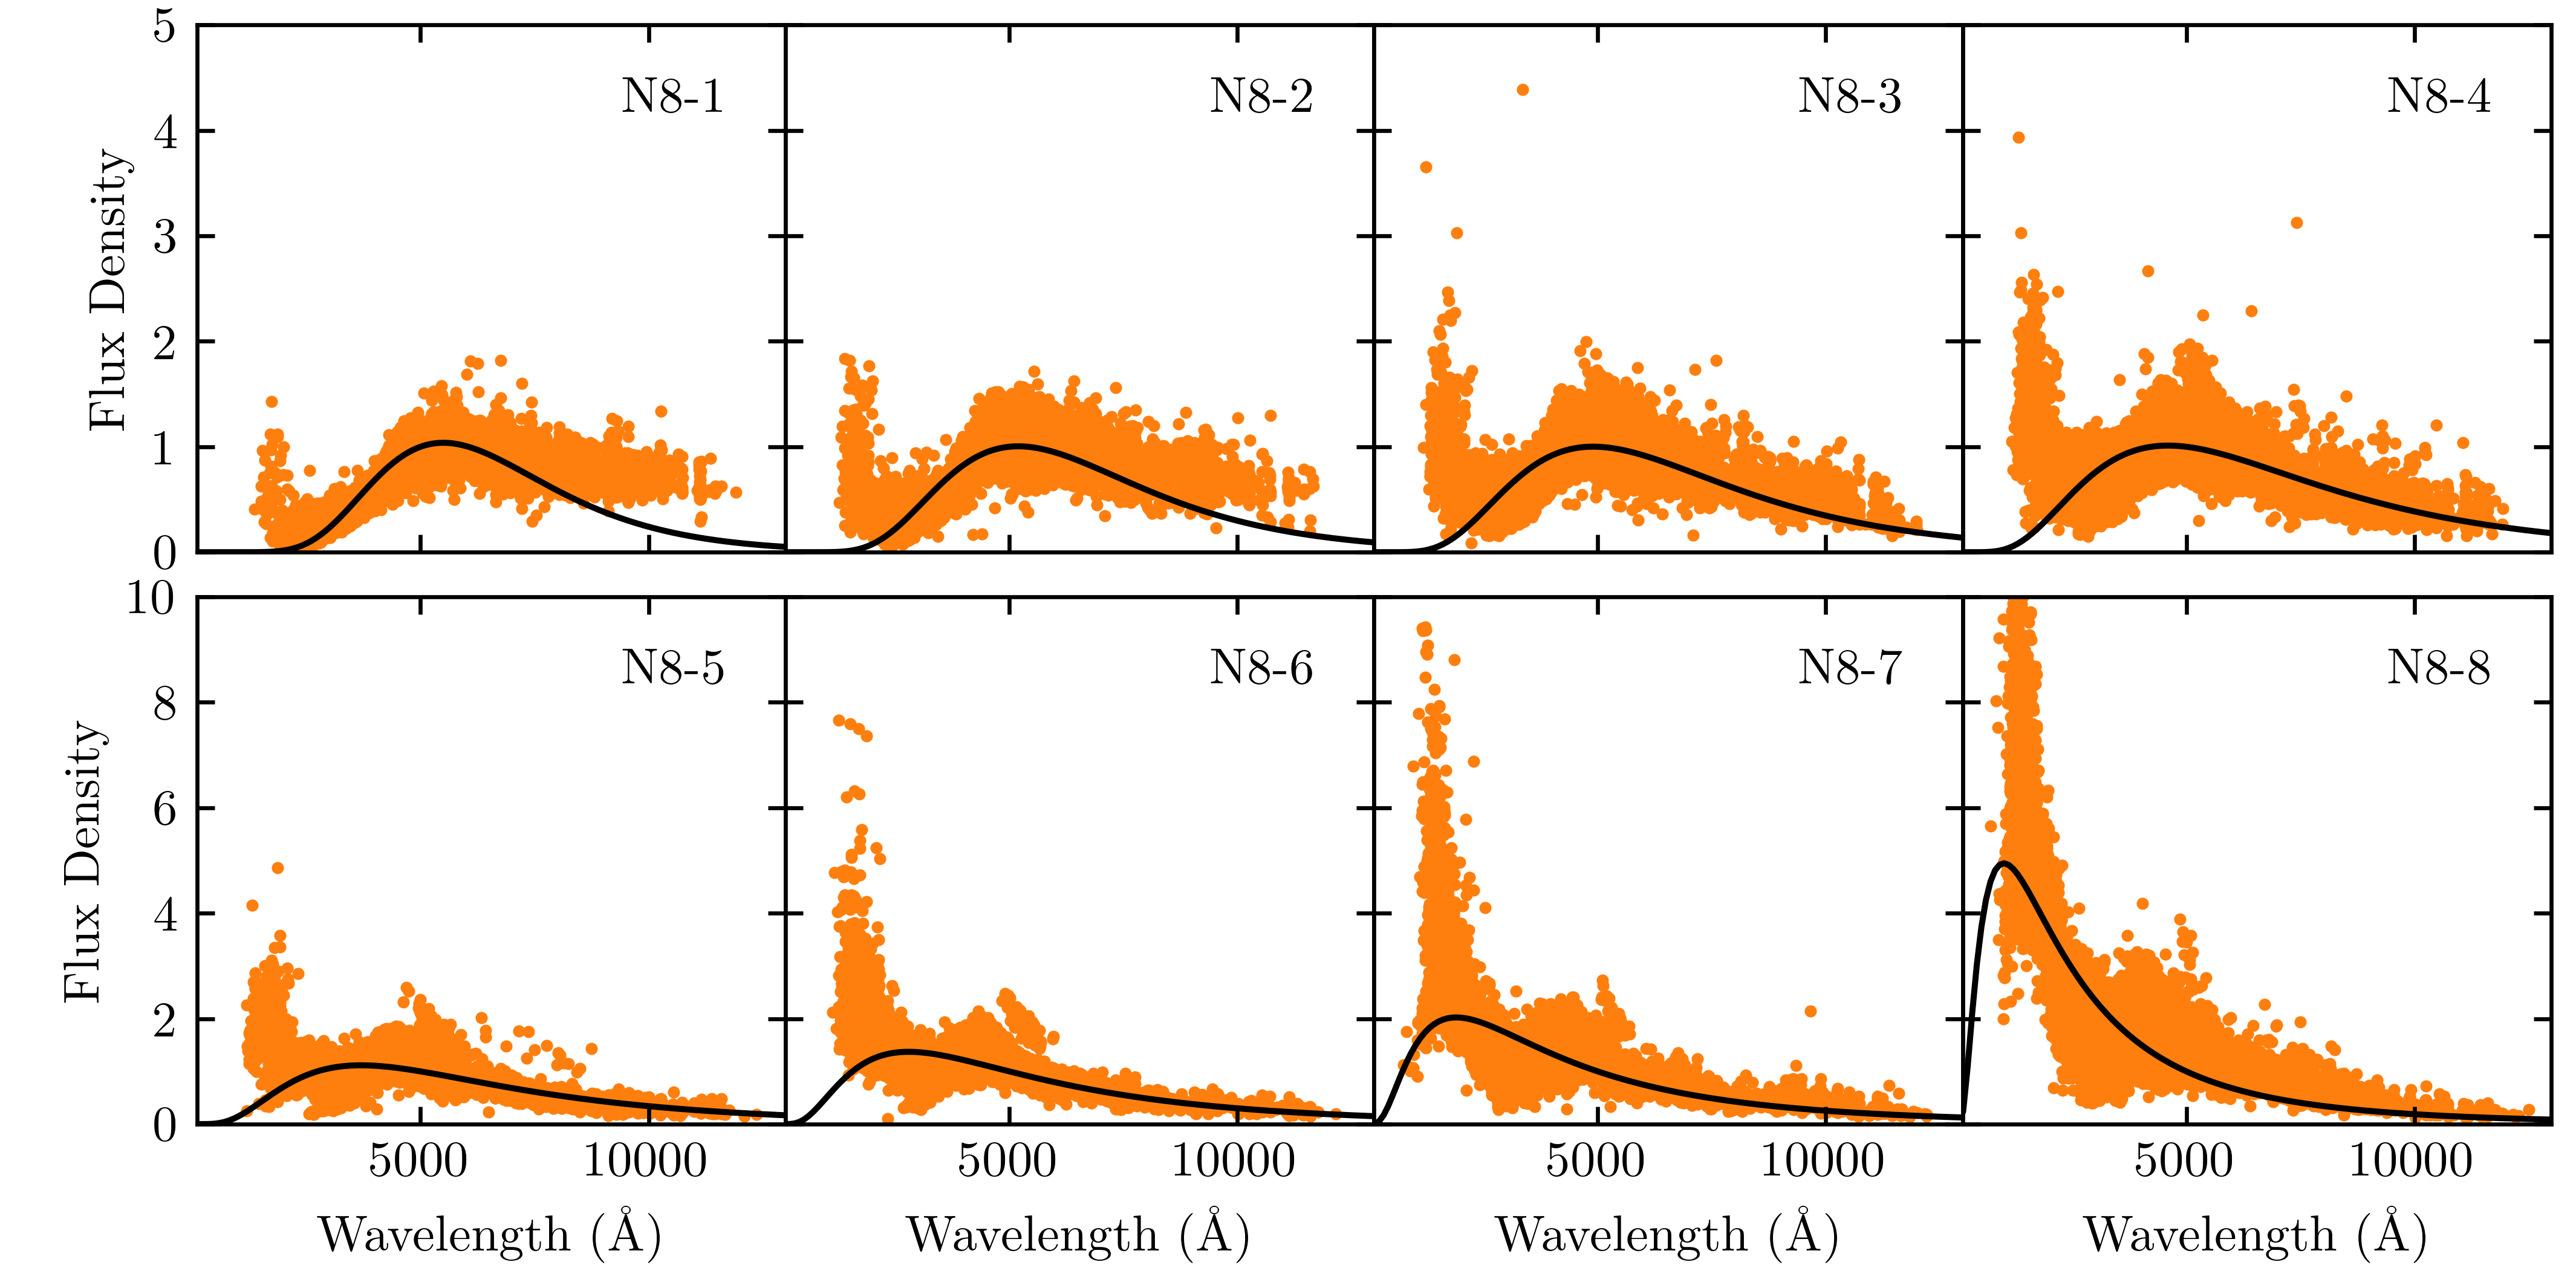
\includegraphics{figures/N8_untrained.png}
    \caption{The untrained N8 templates (black lines) with their original training sets (orange points). N8 1 is the reddest template, with each successive template getting bluer.}
    \label{fig:N8_untrained}
\end{figure*}

These eight templates were chosen to approximately separate the galaxy photometry into distinct groups based on spectral shape, and to ensure that each template had a sizeable and well distributed training set. 
While this requires some guess and check with the assembled training sets, the strength of this method is that you do not need a priori information of galaxy spectra.

After the training sets are assembled, outliers are removed by means of an Isolation Forest in the flux-wavelength space. 
Outliers are determined on a per-flux basis instead of per-galaxy. 
Removing outliers before training the templates helps stabilize the results of the perturbation algorithm described in the next section.

The training algorithm is applied to the N8 templates, resulting in the final templates seen in Figure \ref{fig:N8_trained}. 
The templates were trained for five rounds, with each round consisting of three perturbations with $w=0.5$. 
After the training, the templates more closely resemble real galaxy spectra. 
You can see there are now features in the templates at a much higher resolution than the broadband filters. 
\note{Add lines to guide the eye for 400nm break and spectral lines, where they are visible. Mention those here as well.}

\begin{figure*}
    \centering
    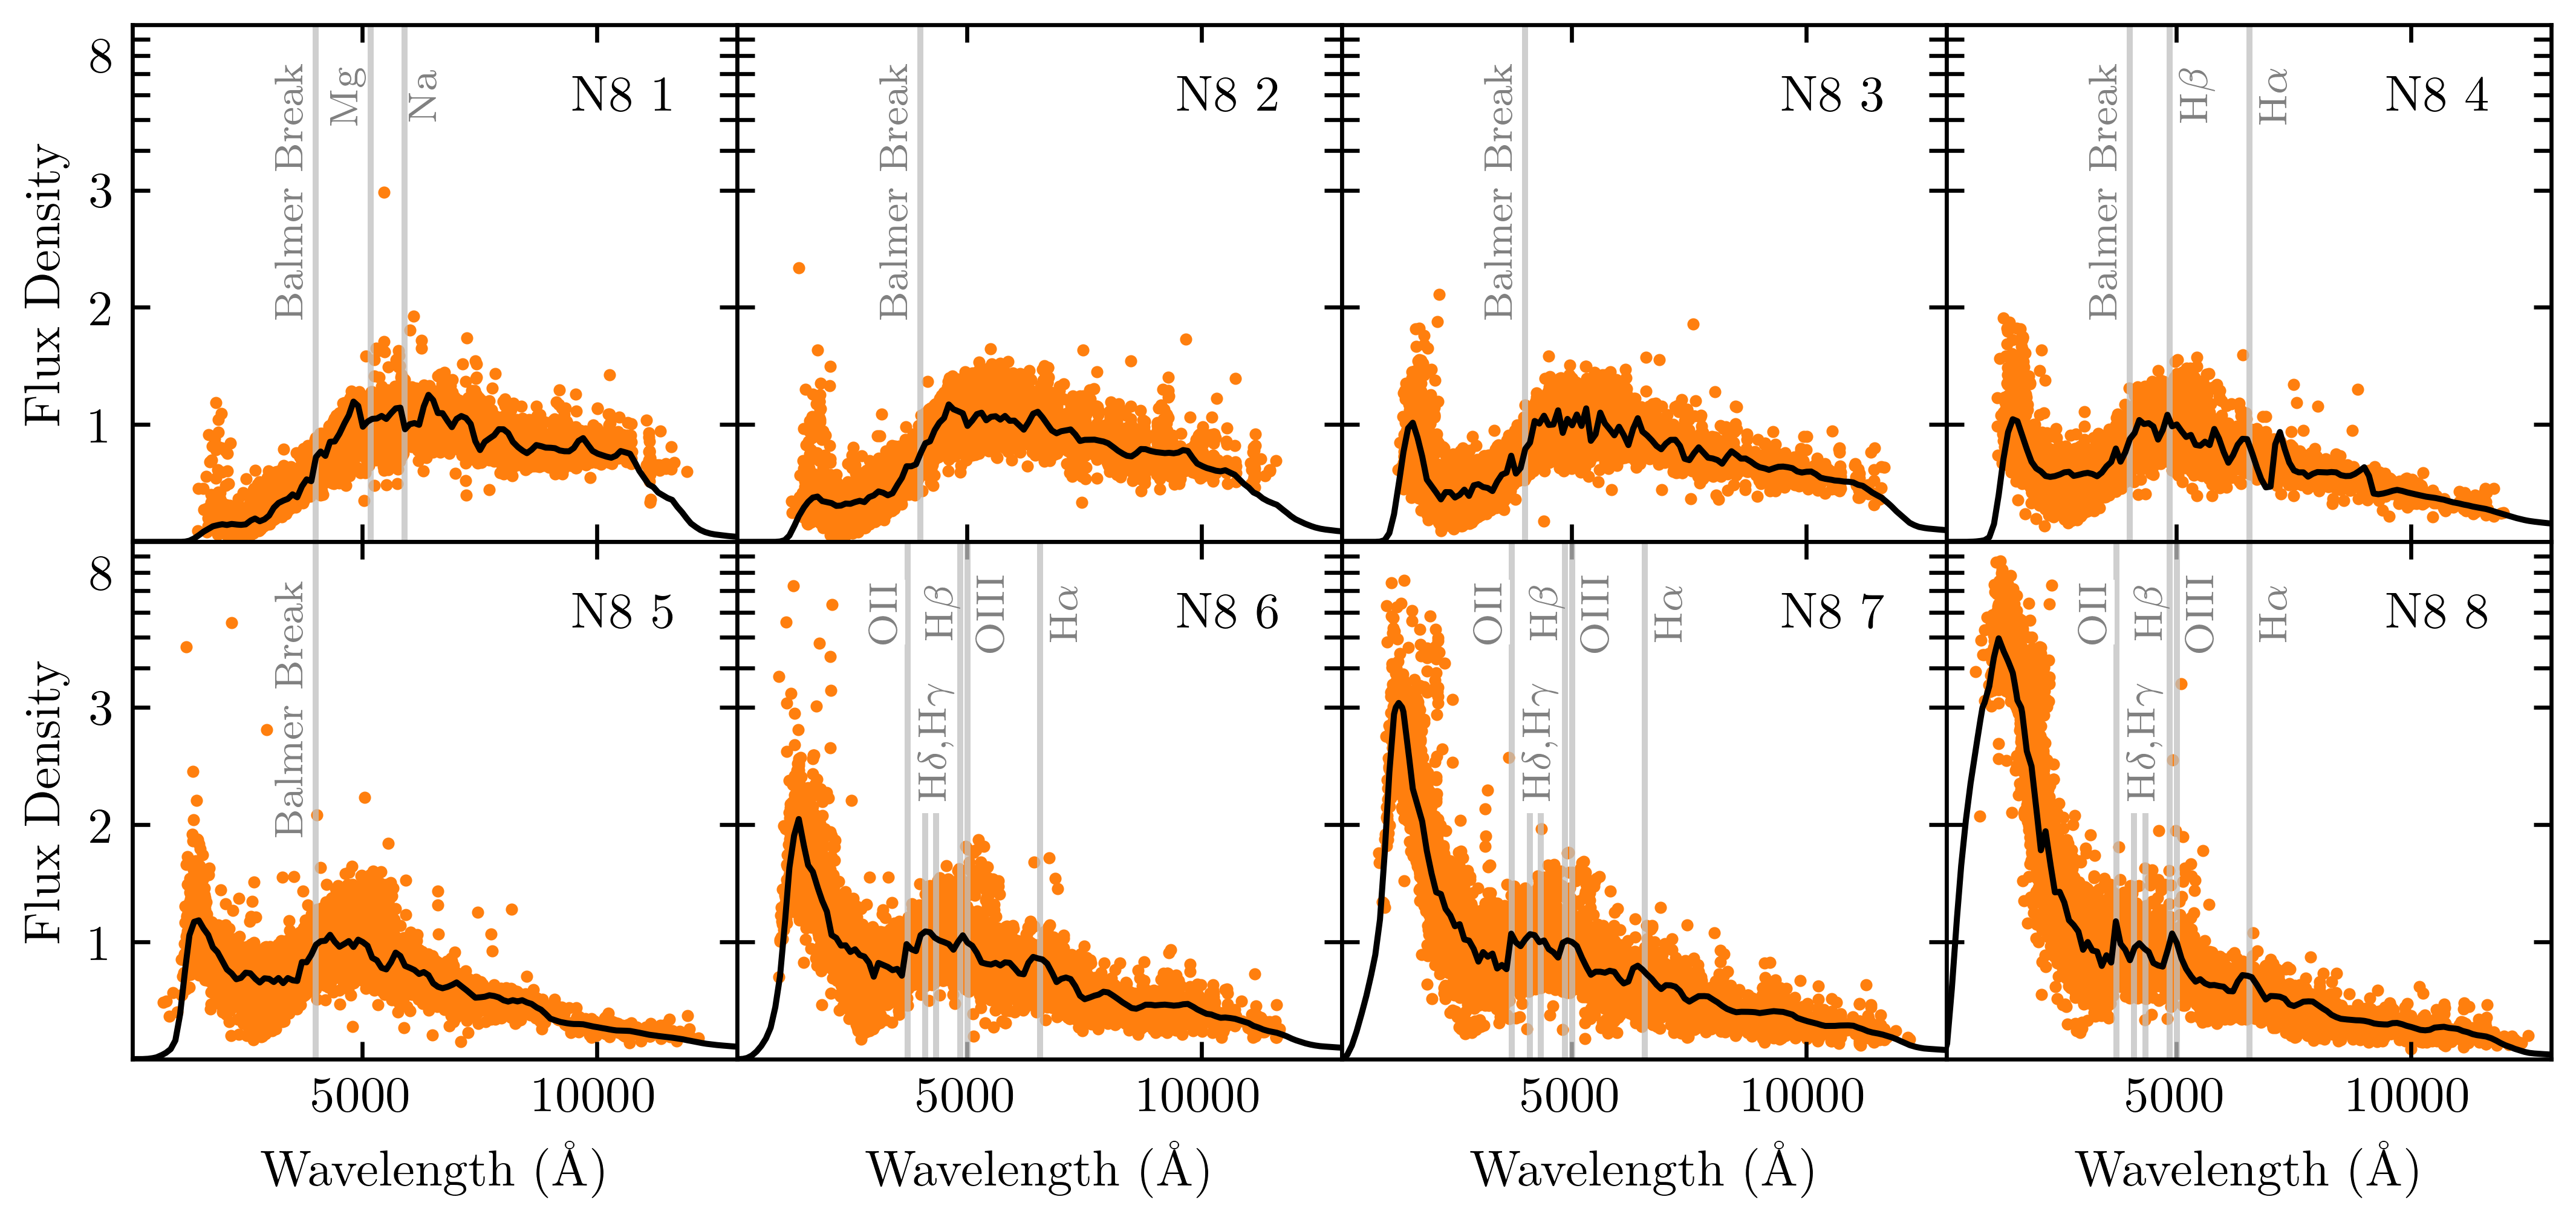
\includegraphics{figures/N8_trained.png}
    \caption{The trained N8 templates (black lines) with their final training sets (orange points). N8 1 is the reddest template, with each successive template getting bluer. \note{Say something about the lines added to guide the eye to spectral features.}}
    \label{fig:N8_trained}
\end{figure*}

In addition to these eight templates, we also train a set of 16 templates from the same range of parameters for the log-normal distribution, creating a more gradual transition of the templates from red to blue. 
This template set (hereafter N16) can be seen with the final training sets in Figure \ref{fig:N16_trained}. 
These were again trained for five rounds, with each round consisting of three perturbations with $w=0.5$. 

\begin{figure*}
    \centering
    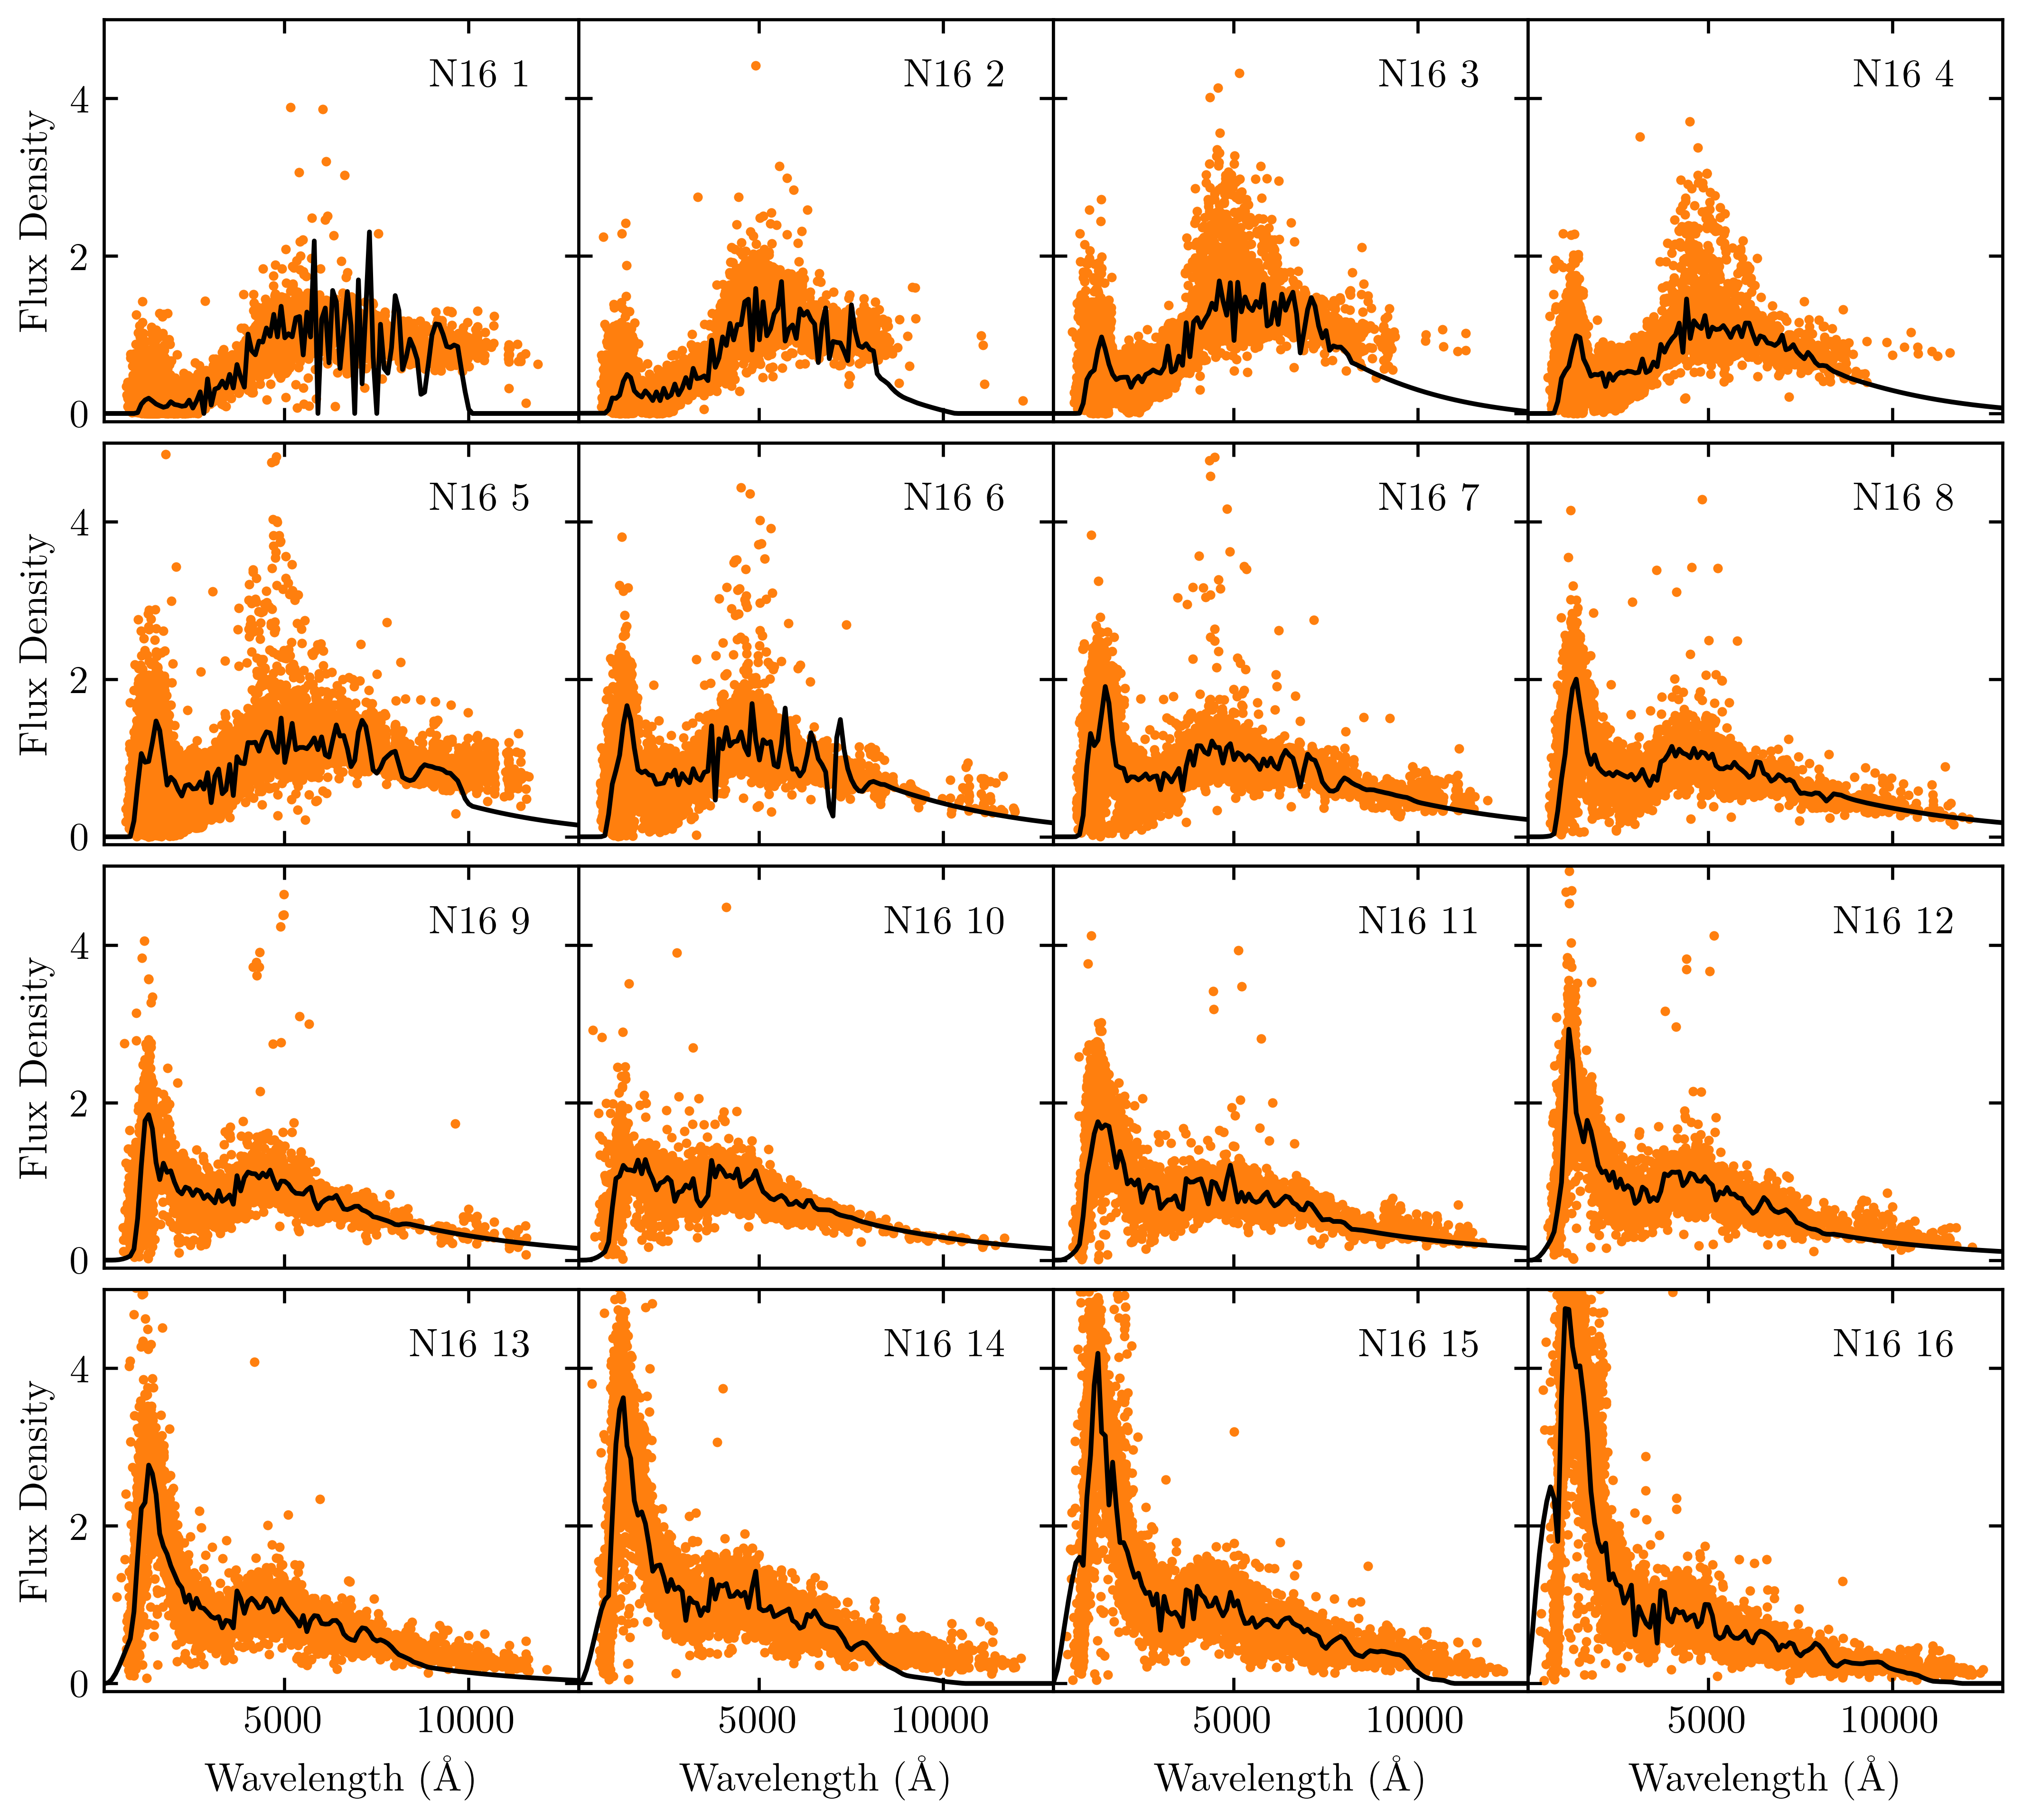
\includegraphics{figures/N16_trained.png}
    \caption{The trained N16 templates (black lines) with their final training sets (orange points). N16 1 is the reddest template, with each successive template getting bluer. \note{Say something about the lines added to guide the eye to spectral features.}}
    \label{fig:N16_trained}
\end{figure*}

In addition to starting from naive templates, one can start with templates derived from spectral synthesis models or observations of local galaxy spectra. 
Here we apply the training algorithm to a standard set of SED templates that comes with \bpz.
This set (hereafter CWW+SB4) consists of four templates from \citet{Coleman1980a} and two starburst templates from \citet{Kinney1996a}, the latter of which were added to account for faint blue galaxies in the HDF-N. 
These six templates were recalibrated by \citet{Benitez2004a} to correct for systematic differences between the observed and predicted galaxy colors in the HDF-N and other spectroscopic catalogs. 
In addition to these six, CWW+SB4 contains two synthetic starburst templates from \citet{Bruzual2003b}, added by \citet{Coe2006a} to account for even bluer galaxies in the UDF.

These templates were trained for five rounds, with each round consisting of one perturbation with $w=2$. 
The results of the training can be seen together with the original CWW+SB4 templates and the final training sets in Figure \ref{fig:cwwsb4_trained}. 
\note{Say something about how the training added additional high resolution structure to the templates and added a red tilt to Im, SB2, 25Myr, and 5Myr.}

\begin{figure*}
    \centering
    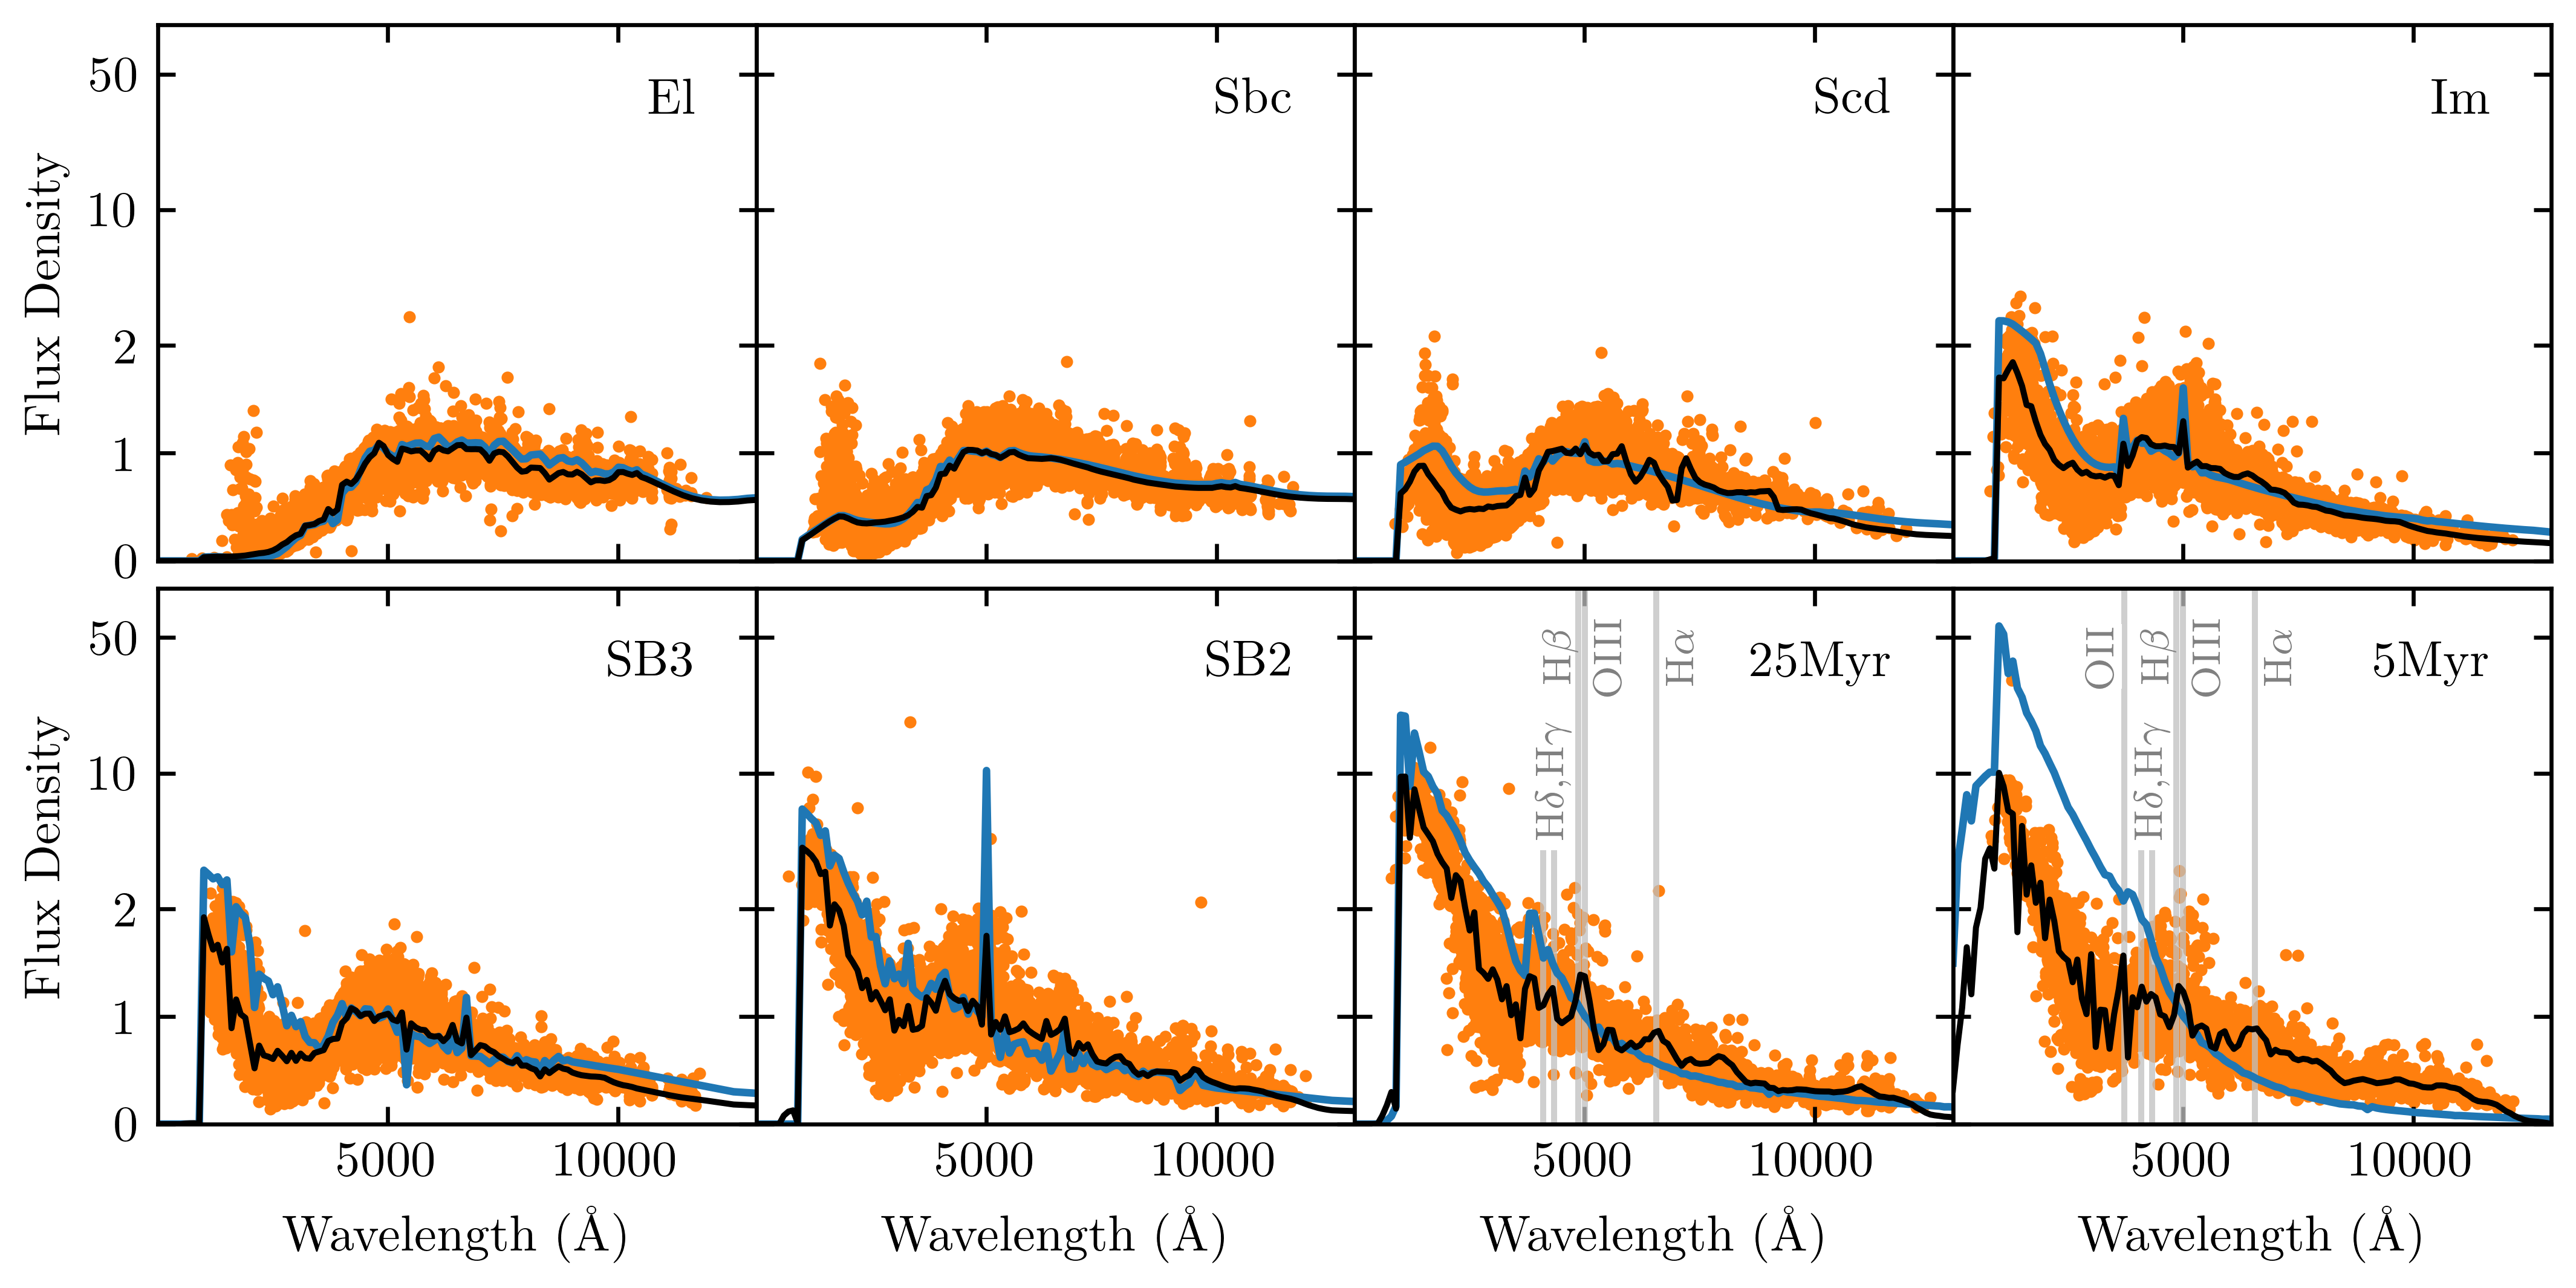
\includegraphics{figures/cwwsb4_trained.png}
    \caption{Result of training the CWW+SB4 templates. The original templates are in blue, the trained templates in black, and the final training sets are displayed as orange points.}
    \label{fig:cwwsb4_trained}
\end{figure*}

% here's a good link for spectral lines
% http://star-www.st-and.ac.uk/~spd3/Teaching/PHYS1002/phys1002_lecture6.pdf
% and here's the spectral ratios
% https://arxiv.org/pdf/1109.2597.pdf